
\subsubsection*{Methodology of the CALREC project}

%4. El detalle de la metodología propuesta en cada uno de los subproyectos participantes, incluyendo la viabilidad metodológica de las tareas. Si fuera necesario, también se incluirá una evaluación crítica de las posibles dificultades de un objetivo específico y un plan de contingencia para resolverlas.
%

{\bf Calibration of SiPMs and PMTs sensors}

The gain and noise of the PMTs and SiPMs sensors will be calibrated with 400 nm LEDs located on the tracking and energy plane. 
%Each SiPM board has a place for one LED.
Calibration data will be acquired during the physics runs.
%During the physics runs, the LEDs will illuminate the chamber at small rate.
The gain and noise will be obtained from a fit to the single photo-electron spectrum.
These parameters will be monitored along time and temperature to correct for possible deviations. 
We expect no difficulties here as we have already used a similar method to calibrate the sensors of NEXT-DEMO.
%We have an experience with this method, as we have used to calibrated the sensors of NEXT-DEMO. 
%This method has been already used to calibrate the sensors of NEXT-DEMO.
%A similar method was already used to calibrate the PMTs of NEXT-DEMO \cite{NEXT-DEMO}. No problems are expected here.

{\bf Energy calibration}

\begin{figure}
\begin{center}
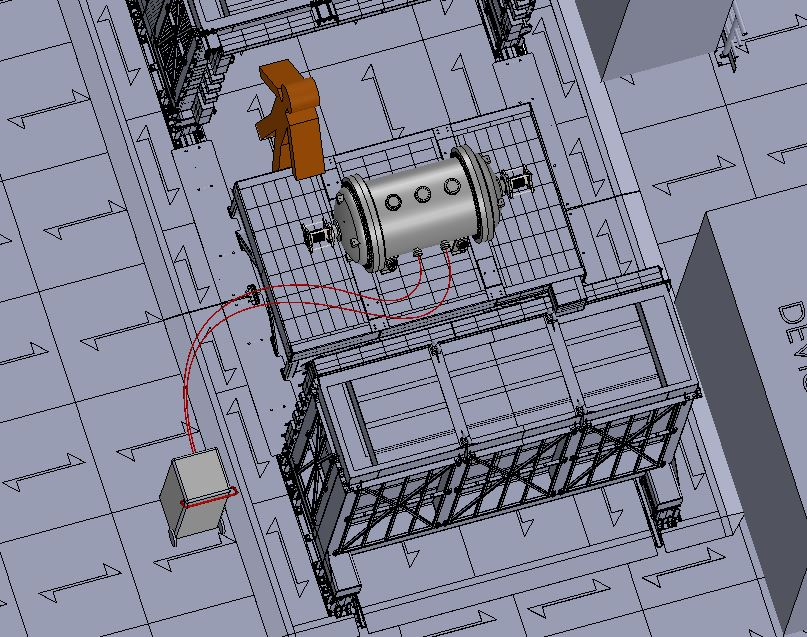
\includegraphics[width=0.5\textwidth]{img/CALREC_LSC_sources.jpg}
%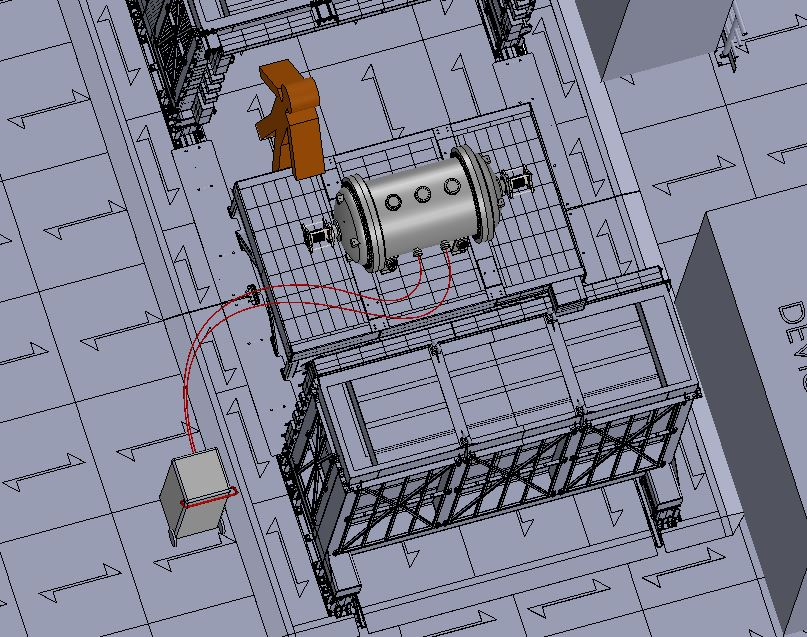
\includegraphics{img/CALIB_LSC_sources.jpg}
\caption{\small Drawing of the NEW detector at the LSC platform where the lead closet with the radioactive sources is on the left. The two guides transfer the high energy gamas into the detector via two ports on the vessel side.}
\label{fig:CALREC_LSC_sources}
\end{center}
\end{figure}

To calibrate in energy, we will use several radiative sources.
In particular  \Tl ~emits a high energy gamma of 2.6 MeV and its double scape peak produces two electrons around 1.6 MeV energy.
The energy resolution and scale will be obtained from the width and position of the 2.6 MeV photo-peak. 
From the two electrons at 1.6 MeV we can estimate the efficiency to identify a \bb ~signal.  
In addition, ~\NA ~(511 keV) and \CS ~(662 keV)  sources will be used to calibrate the energy scale around 500 keV. 
%The sources will be located inside a lead closet on the LSC platform outside the NEXT castle.
%two light guides will direct the gamma rays into the vessel via two ports located on the side. 
In Fig. ~\ref{fig:CALREC_LSC_sources} there is a drawing of the calibration setup at LSC. Radiative sources will be located in a lead shielded closet outside the NEXT castle and two light guides will aim the gammas to two ports on the side of the vessel.  %(see Fig. ~\ref{fig:CALIB_LSC_sources}). 
%Calibration will take place before the start of the run in a periodic basis.
%The detector will be calibrated before we the start of the run and periodically.
%The Calibration procedure itself (security measures,
%Finally, notice 
This is a standard calibration procedure, used in other \bb ~experiments, and no difficulties are expected.
%Calibration run procedures are 
%We are still defining the procedure for the calibration runs (security, time, periodicity and type). This calibration method has been previously used in other \bb experiments (see \cite{COURE-Tl}). We expect no difficulties. 
%A good communication with technical coordinator is essential.
%This part requires that the responsible of the calibration to be frequently at LSC.

{\bf Calibration in position}

Position calibration is needed to correct for the bias on the energy introduced by the geometry of the chamber. According with the results from NEXT-DEMO, for events outside the center region, the PMTs detect less light than expected. To correct for this geometrical bias, we will use X-rays from \Xe ~ (30 keV)  and \KR ~(42 keV). X-rays are point like sources for NEXT and will allow us to map the full active volume. The correction can be obtained from the X-ray energy measurement as a function of $z$ and $x,y$ position. 
%the position on the transverse plane $x,z$.
To have a large statistics sample of X-rays, we plan to introduce \KR ~within the \Xe ~gas.  
\KR~ is produced in the decay of $^{83}$Rb. A piece of zeolite coated with $^{83}$Rb will serve as a source, the free \KR ~will flow into the gas system. \KR ~has a half-life of $1.8 $ hours and it should leave no trace in days. As \KR ~is a pure noble gas, it should not compromise the purity of xenon. 
%The details of the calibration (injection, rates, etc) with \KR~ are still to be defined.
%Most probably NEW will be calibrated with \KR~ before each start of the run.
Successful examples using this calibration exist, nevertheless we will dedicate R+D efforts to test the injection system.
%and study possible secondary effects (as electron attachment).
% NEXT-DEMO prototype could be reused for this propose. 
%Successful examples using this calibration exits in other experiments (\cite{KR}), nevertheless, for contingency, we plan to explore other calibration sources. 

Notice also that X-rays could be used to estimate the Point Spread Function (PSF), the probability that the EL light reach a given SiPM from a point-like source. This function is used by the reconstruction algorithms. With large statistics samples, we can study the PSF as a function of the position on the chamber to correct for possible geometrical distortions. 
%This function a key ingredient for the reconstruction. 
%Algorithms to estimate the PSF from data need to be in place, but no difficulties are expected here.  
 
{\bf Reconstruction algorithms}

The reconstruction algorithms converts the calibrated SiPMs and PMTs signals into a 3D trajectory. 
%Each point of the trajectory has associated a deposited energy. 
%A trajectory is as an electron if a {\it blob} is found in one of the end-points of the trajectory. 
%A \bb ~signal is therefore a trajectory with two blobs.
Algorithms are pieces of C++ code that runs in the official reconstruction program, inside a C++ framework.
The IP of CALREC, in collaboration with F. Ferreiro (IFIC), will coordinate the collaboration efforts to provide the reconstruction algorithms.

\begin{figure}
\begin{center}
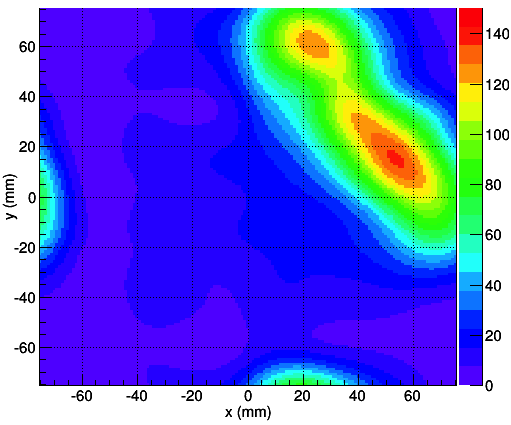
\includegraphics[width=0.5\textwidth]{img/CALREC_slice5muon.png}
%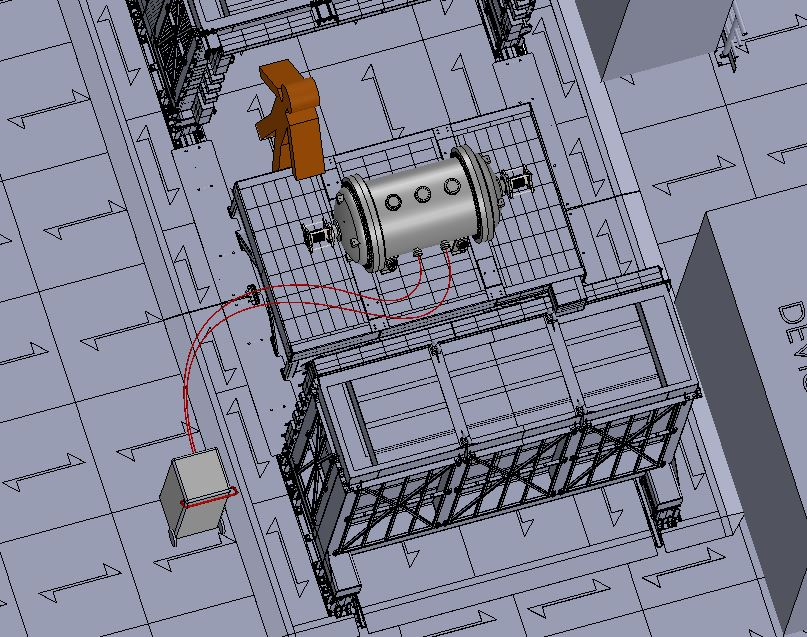
\includegraphics{img/CALIB_LSC_sources.jpg}
\caption{\small Reconstructed image with NEXT-DEMO of a muon candidate crossing parallel to the tracking plane.}
\label{fig:CALREC_muon}
\end{center}
\end{figure}

Three algorithms are currently on place, they are in a primitive state, they run from simple to complex.
The simple one has been developed by the IFIC group for the NEXT-DEMO reconstruction. A collection of SiPMs are clustered together if they meet a given criteria of proximity and signal. A 3D track is obtained with the interpolation between clusters at different $z$ positions. This method is simple and good enough for an initial reconstruction of all events. But it lacks the capability to distinguish complex structures as twists in the transverse plane or vertical tracks. 
A second algorithm has been develop by the USC group. It uses the SiPMs signal and the PSF to recover the image of the electron at the EL plane using a Fast Fourier transform. The method is still in a preliminary stage, but it allows us to recover the transverse plane image. See for example Fig.~\ref{fig:CALREC_muon}, that shows a muon candidate crossing vertically the NEXT-DEMO detector. Next step is to connect the transverse images into a 3D trajectory. This method is fast enough to process a large amount of data and provides the capability of finding complex structures in the transverse plane. 
Te third reconstruction algorithm is been developed by the IFIC group. The full detector volume is divided in small ($5\times5\times5$ mm$^3$) 3D boxes. Using the probability function that associates the deposited energy in a given box with the signal detected at the SiPMs and PMTs, and via an iterative process, the method finds the trajectory that maximizes the likelihood that the detected signal match the image produced by the trajectory. This is a time consuming algorithm but it expected to have the ultimate resolution. Notice nevertheless, that it relies on the accurate estimation of the signal left on the PMTs and SiPMs from a deposition at a given point of the detector. 

We will develop and improve these algorithms to
 have the most accurate reconstruction possible.
Algorithms will be tested using simulated data
% computing time  and performance. 
and they will be validated with real data from the \NA,  ~\CS ~and \Tl ~sources. Similar studies are been carried out with the NEXT-DEMO data.
%This is a crucial step in order to gain credibility with topological signatures.
%The definition of an algorithm requires an effort of success and failure trials to finally get the final version. It also requires a detailed comparison data/simulation and validation. This is intelectual challenge, there are no technological problems expected.

\begin{figure}
\begin{center}
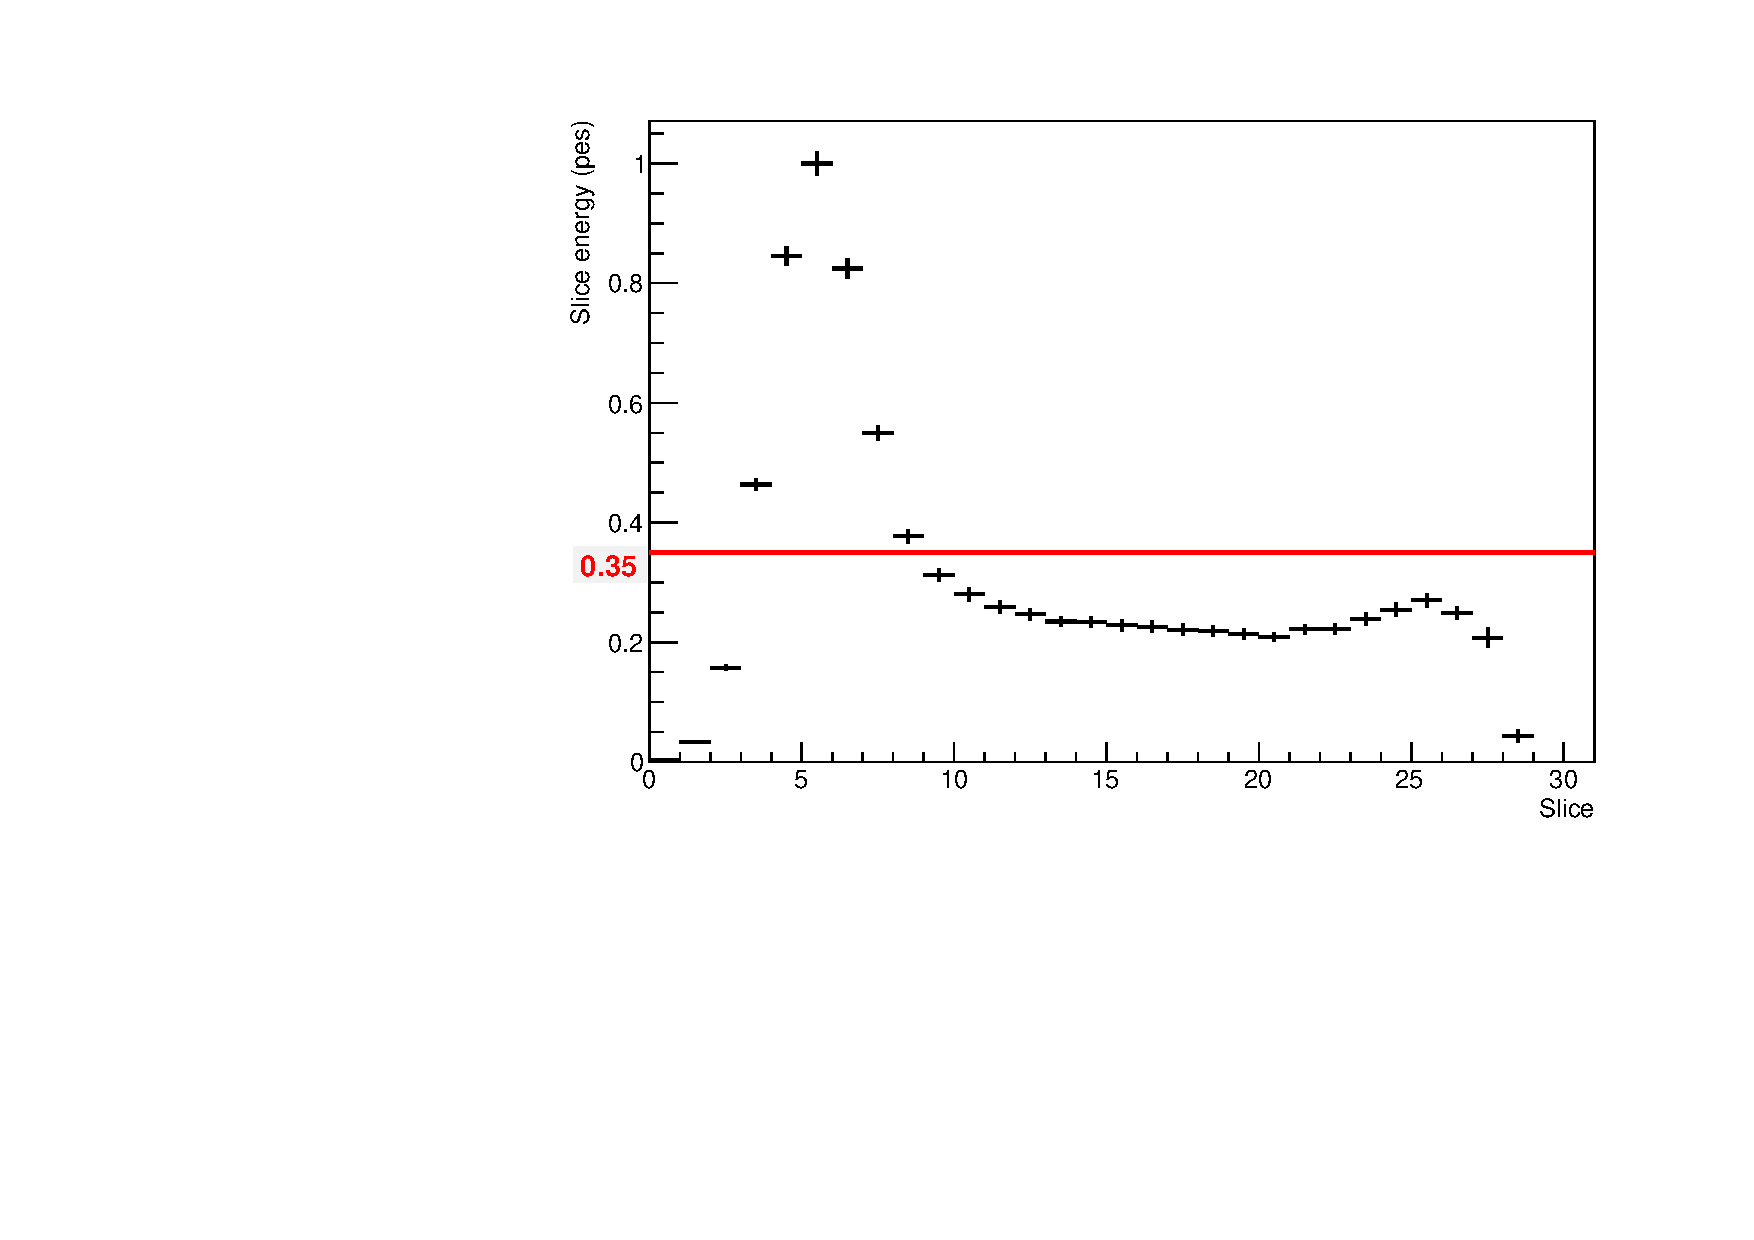
\includegraphics[width=0.5\textwidth]{img/CALREC_Eslice_DEMO.pdf}
%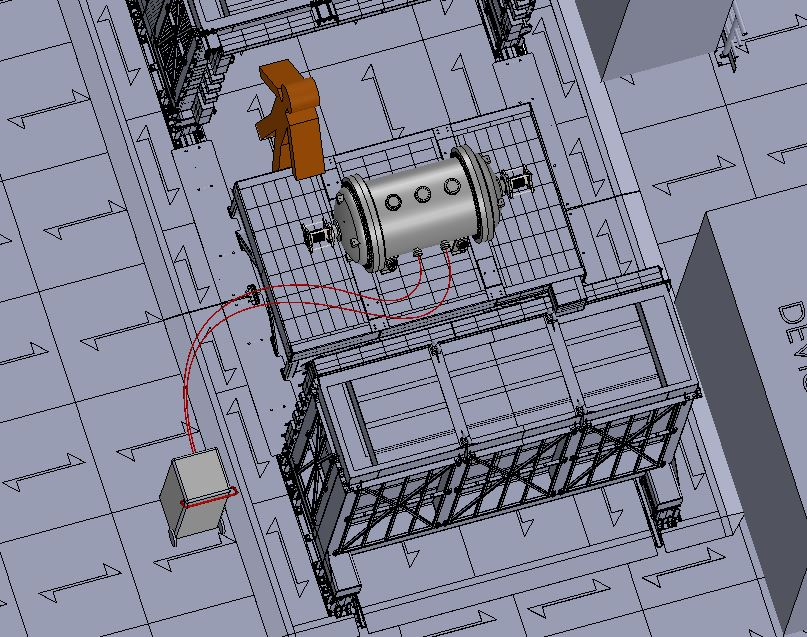
\includegraphics{img/CALIB_LSC_sources.jpg}
\caption{\small Average energy (in arbitrary units) of horizontal electrons vs time slice from 511 keV \NA ~gamma interactions in NEXT-DEMO. The electron and blob parts are clearly visible, above and below the red line.}
\label{fig:CALREC_E}
\end{center}
\end{figure}

An electron track in NEXT ends with a large deposited energy (blob) after the Bragg peak, while a \bb ~signature, two electrons, is a track with two blobs at the ends.
This is the unique topological discriminant signature of NEXT.
Fig.  ~\ref{fig:CALREC_E} shows the average energy profile for horizontal 511 keV electrons moving towards the anode. It has been obtained with NEXT-DEMO \NA ~events. The mip and blob electrons parts are clearly visible. This is on average, but event by event, there are large energy fluctuations. 
The validation of a blob identification algorithms will be performed on the calibration data, in particular with the 2.6 MeV \Tl~ photo-peak and the two electrons from the double scape peak. This is a crucial ingredient to understand the topological capabilities of NEXT.
% therefore a sophisticated selection needs to be defined. This will require the use of multivariate techniques and detailed studies of the blob structure with simulation and calibration data.
%Therefore, the blob-selection algorithm requires validation.
%Remember that the \Tl ~photo-peak signal (2.6 MeV) is a great candle to estimate the efficiency of the blob-identification algorithm. Furthermore, the double-peak scape (1.6 MeV) provides two electrons, that allow us to estimate the efficiency of identifying two blobs. 

{\bf \bb ~Analysis}

The measurement of the \bb ~spectrum follows standard methods on HEP. It has tree steps: definition of the signal region (region of interest), estimation of the contamination events on that region and a fine study of systematic uncertainties. Large MC samples will be used to define the signal selection.
The analysis will be performed in a 2D plane, one axis will be the energy and the other the output of a multi-variate tehcnique (such as Neural Network or Boosted Decision Trees) that will combine the topological information into one single variable. This variable will be calibrated with the \Tl ~peak and the double scape peak; and the energy with the \Tl ~peak, as previously mentioned. The energy spectrum from the contamination processes will be obtained from detailed studies, in particular from the simulation of the radio contamination sources in the detector material that have been measured by the radio-purity group.

%The efficiency of the selection and the contamination levels will be estimated from data, using the \Tl ~two-electrons from the doble scape peak at ~1.6 MeV and the photo-peak at 2.6 MeV, as commented before. The energy scale and resolution will be estimated using the 2.6 MeV \Tl ~photo-peak. The expected energy spectrum of the detector will be obtained from the radio purity measurements in conjunction with the detector simulation. Uncertainties on the spectrum around the region of interest will be carefully estimated.
A fit to the energy spectrum with all the components will allow us to determine the \bb ~decay yield and measure its life-time.
%The yield of \bb~ events will be obtained from the fit and used to measure the life-time of this process. 
%It has been already measured by EXO-200 \cite{EXO} and KamLAND-Zen \cite{KAMLAND}.
%This measurement is a mayor milestone of the NEXT collaboration. 
This measurement will confirm the capabilities of NEXT and will provide an accurate estimate, based on data, of the sensitivity of NEXT-100 and NEXT 1 ton detectors. 

The \bbonu ~search to be perform with NEXT-100 data is similar to the described above. The signal energy distribution could be estimated again from \Tl ~2.6 MeV peak. Finally, the energy spectrum will be fit to all contributions, including the \bbonu ~signal.
%From the estimated yield and detection efficiency, we could them measure, or set a limit in, the life-time on the \bbonu decay.

{\bf R+D with gas mixtures within the \BATA ~subproject}

%Within this project the USC will participate into the R+D efforts of NEXT. 
NEXT collaboration have preliminary results on the uses of additives to improve the tracking reconstruction. Additives, such as TMA, reduce the electron diffusion, increase the drift velocity and transfer energy to scintillation light at 300 nm (easier to detect than the one of Xenon, 170 nm). These additives could in addition, favor the transition of $Ba^{++}\to Ba^+$ by quenching effects. USC will contribute to study the effects of different additives and concentrations, in particular in which condition they favor the $Ba^{++}$ transition.
These studies will be performed reusing previous prototypes and in collaboration with the IFIC, UZ (Zaragoza) and CLPU groups.
%Preliminary results have been published by the NEXT collaboration \cite{NEXT-TMVA}. The R+D should be focus on the handling of the mixtures and the study of the detector performance as function of additive concentration and pressure. This studies could be done with the NEXT prototypes of UZ.
%The second R+D line could result in an excellent synergy between \bb and dark matter detectors. Electrons from ionization produced by a nuclear recoil, could recombine different depending on the angle between the recoil and the electric field. As the dark matter should be a flux with a privileged direction, we could determine an excess on that direction (see \cite{NEXT-DM-1}). Preliminary studies at \cite{NEXT-DM} are promising. Further studies are needed to proof this detector concept. This R+D could be done in collaboration with the Berkeley group.
%The third R+D line is the \BATA proposal, of tagging the Ba product of the \bbonu decay with lasers exploiting the convenient atomic levels. This is a challenging proposal to be carried out in collaboration in collaboration with the Center for Pulsed Lasers (CLPU) at Salamanca. 

 


